\graphicspath{{../../S10_Comparaison_et_egalite_de_fractions/Images/}}

\themeN
\chapter{Comparaison et égalité de fractions} \label{S10}

\programme%
   {\item Fractions, nombres rationnels.
   \item Égalité de fractions.
   \item Ordre sur les nombres rationnels.}
   {\item Comparer, ranger, encadrer des nombres fractionnaires.
   \item Repérer et placer un nombre rationnel sur une droite graduée.}

\vfill

\begin{debat}{Débat : les fractions, ces nombres rompus !}
   Tout nombre peut s'écrire de différentes façons : ils ont des habillages différents mais ont la même valeur. La façon dont on les écrit permet de pouvoir les comparer. Par exemple, la {\bf fraction} $\dfrac68$ possède (entre autres) les représentations suivantes :
   \tcblower
      {\psset{unit=0.8}
      \begin{pspicture}(-4,-4)(4,4)  
         {\large
         \multido{\n=5+60,\i=55+60}{6}{\psline(3;\n)(0,0)(3;\i)}
         \multido{\n=30+60,\i=-60+60,\r=120+60}{6}{\psarc(2.719;\n){1.268}{\i}{\r}}
         \pscircle[fillstyle=solid,fillcolor=yellow](0,0){1.3}
         \rput(0,0){\bf $\dfrac68$}
         \rput(2.7;30){75\,\%}
         \rput(2.7;-30){0,75}
         \rput(2.7;150){$\dfrac34$}
         \rput(2.7;-150){$\dfrac{75}{100}$}
         \rput(2.7;90){\pswedge[fillstyle=solid,fillcolor=Crimson](0,0){0.8}{0}{-90}
                              \pscircle(0,0){0.8}
                              \multido{\n=0+45}{8}{\psline(0,0)(0.8;\n)}}
         \rput(2.7;-90){\psline(-1,0)(1,0)  
         \rput(-1,-0.4){\footnotesize 0}
         \rput(1,-0.4){\footnotesize 1}
         \psline[linecolor=Crimson,linewidth=1mm](-1,0)(0.5,0) \multido{\r=-1+0.25}{9}{\rput(\r,0){|}}}}
      \end{pspicture}}
\end{debat}

\hfill {\gray Vidéo : \href{https://www.youtube.com/watch?v=eawBr43xWf8}{\bf Les fractions}, chaîne Youtube {\it Petits contes mathématiques}.}


%%% Approche %%%
\begin{Maquette}[Cours]{Theme={Activité d'approche},Couleur={SteelBlue}}

   \AAtitre{Des briques et des fractions}

      {\it Objectifs : utiliser des fractions pour exprimer une proportion ; produire des fractions égales, ranger des fractions.}

      \begin{AActivite}

         \AApartie{Les Lego®}
            \begin{minipage}{10cm}
               On choisit la brique de Lego® classique $u$ ci-contre que l'on prend comme unité et les onze briques $a$ à $k$. \par
               On considère que le volume d'une brique est proportionnel au nombre de \og boutons \fg{} présents sur le dessus.
            \end{minipage}
            \hspace{1cm}
            \begin{minipage}{5cm}
               $u$ : 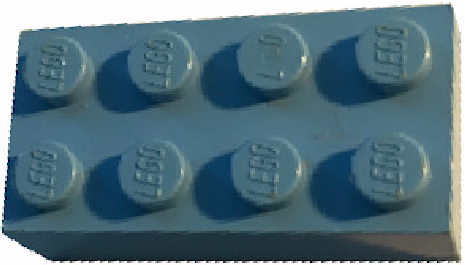
\includegraphics[width=3.15cm]{lego_4_2a}
            \end{minipage} \par \bigskip
               $a$ : 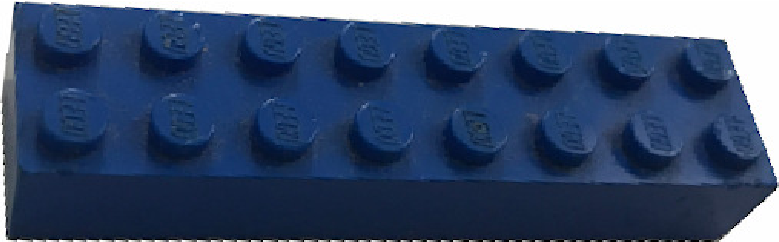
\includegraphics[width=5.22cm]{lego_8_2a} \qquad 
               $b$ : 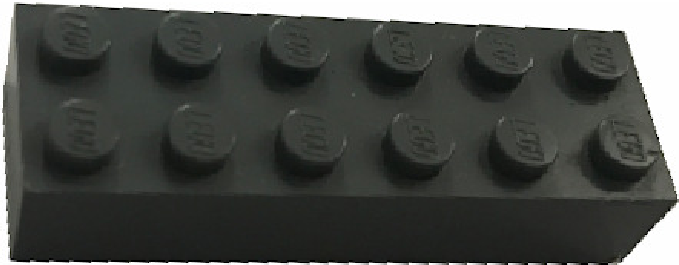
\includegraphics[width=3.6cm]{lego_6_2a} \qquad
               $c$ : 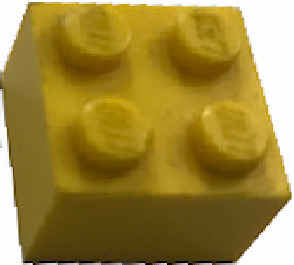
\includegraphics[width=1.35cm]{lego_2_2a} \qquad
               $d$ : 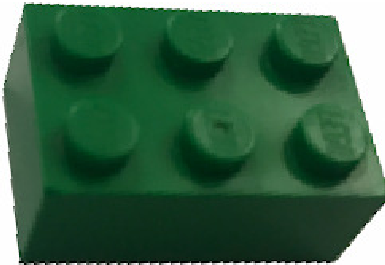
\includegraphics[width=1.8cm]{lego_3_2a} \\ [5mm]
               $e$ : 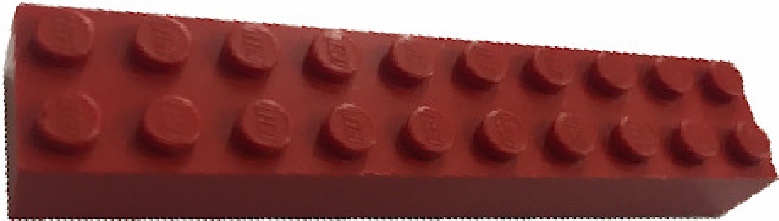
\includegraphics[width=6.3cm]{lego_10_2a} \qquad
               $f$ : 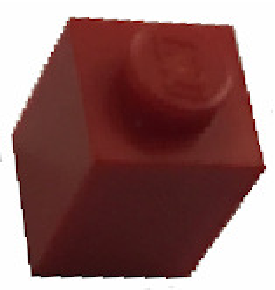
\includegraphics[width=0.9cm]{lego_1_1a} \qquad
               $g$ : 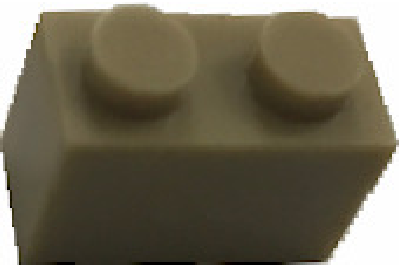
\includegraphics[width=1.35cm]{lego_2_1a} \qquad
               $h$ : 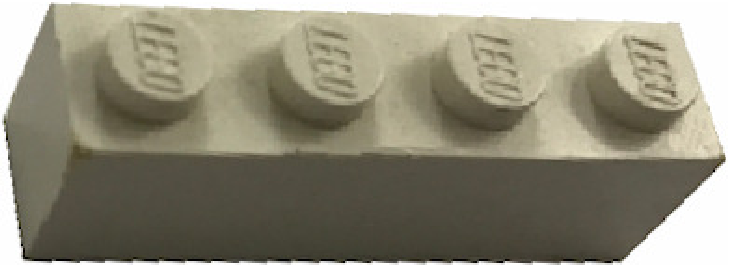
\includegraphics[width=2.7cm]{lego_4_1a} \\ [5mm]
               $i$ : 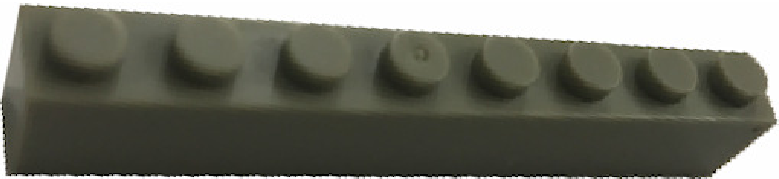
\includegraphics[width=5.4cm]{lego_8_1a} \qquad
               $j$ : 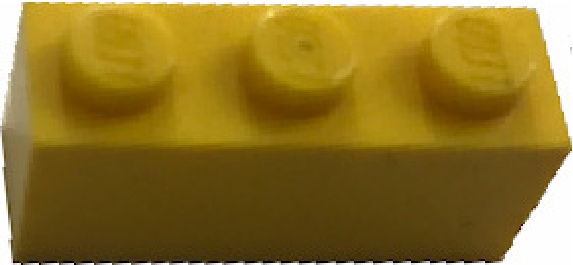
\includegraphics[width=1.98cm]{lego_3_1a} \qquad
               $k$ : 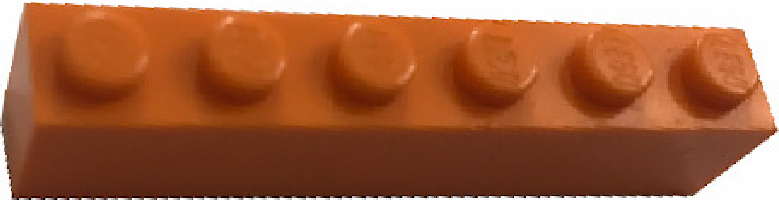
\includegraphics[width=4.05cm]{lego_6_1a} \bigskip
               
         \AApartie{Les fractions}
            \begin{enumerate}
               \item Compléter les égalités suivantes à l'aide de nombres fractionnaires : \par \bigskip
                  \begin{multicols}{6}
                     $a = \pointilles u$ \par \vskip8mm
                     $g = \pointilles u$ \par \vskip8mm
                     $b = \pointilles u$ \par \vskip8mm
                     $h = \pointilles u$ \par \vskip8mm
                     $c = \pointilles u$ \par \vskip8mm
                     $i = \pointilles u$ \par \vskip8mm
                     $d = \pointilles u$ \par \vskip8mm
                     $j = \pointilles u$ \par \vskip8mm
                     $e = \pointilles u$ \par \vskip8mm
                     $k = \pointilles u$ \par \vskip8mm
                     $f = \pointilles u$ \par \vskip8mm
                  \end{multicols} \vskip8mm
               \item Compléter les égalités suivantes à l'aide de fractions dont le dénominateur est 8 : \par \bigskip
                  \begin{multicols}{6}
                     $a = \dfrac{\pointilles[1cm]}{8} u$ \par \vskip8mm
                     $g = \dfrac{\pointilles[1cm]}{8} u$ \par \vskip8mm
                     $b = \dfrac{\pointilles[1cm]}{8} u$ \par \vskip8mm
                     $h = \dfrac{\pointilles[1cm]}{8} u$ \par \vskip8mm
                     $c = \dfrac{\pointilles[1cm]}{8} u$ \par \vskip8mm
                     $i = \dfrac{\pointilles[1cm]}{8} u$ \par \vskip8mm
                     $d = \dfrac{\pointilles[1cm]}{8} u$ \par \vskip8mm
                     $j = \dfrac{\pointilles[1cm]}{8} u$ \par \vskip8mm
                     $e = \dfrac{\pointilles[1cm]}{8} u$ \par \vskip8mm
                     $k = \dfrac{\pointilles[1cm]}{8} u$ \par \vskip8mm
                     $f = \dfrac{\pointilles[1cm]}{8} u$ \par \vskip8mm
                  \end{multicols} \vskip8mm
               \item Classer les Lego® dans l'ordre croissant de leur volume : \par \vskip5mm
                  \pointilles \par \vskip7mm
                  \pointilles \par \bigskip
         \end{enumerate}

   \end{AActivite}

\end{Maquette}


%%%Trace écrite %%%
\begin{Maquette}[Cours]{Theme={Trace écrite},Couleur={0.4[SteelBlue,Black]}}

   %%%1
   \section{Égalité de fractions}

      \begin{propriete*}{}
         On ne change pas la valeur d'une fraction en multipliant ou en divisant le numérateur et le dénominateur par un même nombre relatif non nul.
         $$\dfrac{b}{c} =\dfrac{b\times a}{c\times a}= \dfrac{ba}{ca}. \text{\quad On a aussi \quad }a\times\dfrac{b}{c}= \dfrac{a\times b}{c} =\dfrac{ab}{c}$$
      \end{propriete*}

      Démonstration :\qquad
         {\hautab{1.7}
         \begin{tabular}{p{4cm}p{10cm}}
            $(a\times c)\times\dfrac{b}{c} =a\times \left(c\times\dfrac{b}{c}\right)$
            &
            {\it associativité de la multiplication} \\
            $(a\times c)\times\dfrac{b}{c} =a\times b$
            &
            {\it $\dfrac{b}{c}$ est le nombre qui, multiplié par $c$ donne $b$ donc $c\times\dfrac{b}{c} =b$} \\
            donc, $\dfrac{b}{c} =\dfrac{a\times b}{a\times c}$
            &
            {\it puisque $\dfrac{a\times b}{a\times c}$ est le nombre qui, multiplié par $a\times c$ donne $a\times b$} \\
         \end{tabular}}

      \begin{exemple*}{}   
         $$\dfrac12 =\dfrac{1\times2}{2\times2} =\dfrac24 =\dfrac{2\times2}{4\times2} = \dfrac48\dots \qquad ; \qquad 7\times\dfrac{3}{5} =\dfrac{7\times3}{5} =\dfrac{21}{5}$$
      \end{exemple*}

      Remarque : la propriété permet de {\bf simplifier} des fractions, ce qui  signifie écrire une fraction qui lui est égale, mais avec un numérateur et un dénominateur plus petits.

      \begin{exemple*}{}
         Pour simplifier $\dfrac{150}{180}$, on peut diviser le numérateur et le dénominateur par 10 : $\dfrac{150}{180} =\dfrac{150\div10}{180\div10} =\dfrac{15}{18}$ \par \smallskip
         puis les diviser encore par 3 : $\dfrac{15}{18} =\dfrac{15\div3}{18\div3} =\dfrac56$.
      \end{exemple*}


   %%%2
   \section{Comparaison de fractions}

      \begin{methode*}{Comparer des fractions}
         Pour comparer deux fractions ayant le même dénominateur, il suffit de comparer les numérateurs : la fraction ayant le plus grand numérateur est la plus grande.
         \begin{exmethode}
            Comparer $\dfrac26$ et $\dfrac36$ \; : \; \parbox{1.4cm}{\Fraction[Rayon=6mm,Couleur=SteelBlue,Reponse]{2/6}} et \; \parbox{1.2cm}{\Fraction[Rayon=6mm,Couleur=SteelBlue,Reponse]{3/6}}
            \tcblower
               $2<3$ donc $\dfrac26<\dfrac36$
         \end{exmethode}
         Pour comparer deux fractions de dénominateurs multiples, on modifie l'écriture de l'une des fractions pour qu'elle ait le même dénominateur que l'autre.
         \begin{exmethode}
            Comparer $\dfrac23$ et $\dfrac{7}{12}$ \; : \; \parbox{1.4cm}{\Fraction[Rayon=6mm,Couleur=SteelBlue,Reponse]{2/3}} et \; \parbox{1.2cm}{\Fraction[Rayon=6mm,Couleur=SteelBlue,Reponse]{7/12}}
            \tcblower
               $\dfrac23=\dfrac{2\times4}{3\times4}=\dfrac{8}{12}$ \; : \; \parbox{1.4cm}{\Fraction[Rayon=6mm,Couleur=SteelBlue,Reponse]{2/3}} = \; \parbox{1.2cm}{\Fraction[Rayon=6mm,Couleur=SteelBlue,Reponse]{8/12}} \par \medskip
               $\dfrac{8}{12}>\dfrac{7}{12}$ donc, $\dfrac23>\dfrac{7}{12}$ \; : \; \parbox{1.4cm}{\Fraction[Rayon=6mm,Couleur=SteelBlue,Reponse]{8/12}} > \; \parbox{1.2cm}{\Fraction[Rayon=6mm,Couleur=SteelBlue,Reponse]{7/12}}
         \end{exmethode}
      \end{methode*}

\end{Maquette}


%%% Exercices %%%
\begin{Maquette}[Fiche,CorrigeFin,Colonnes=2]{}
   
   \begin{multicols}{2}

      \begin{exercice}[SLF] %1
         Écrire la fraction qui représente la partie colorée de chaque figure puis la simplifier si possible.
         \begin{center}
            a \Fraction[Regulier,Cotes=4,Rayon=6mm,Couleur=Cyan,Reponse]{1/4} \quad b \Fraction[Regulier,Cotes=4,Rayon=6mm,Couleur=Cyan,Reponse]{3/4} \quad c \Fraction[Regulier,Cotes=4,Rayon=6mm,Couleur=Cyan,Reponse]{2/4} \quad d\Fraction[Regulier,Cotes=4,Rayon=6mm,Couleur=Cyan,Reponse]{4/4} \par \bigskip
            e \Fraction[Rayon=6mm,Couleur=IndianRed,Reponse]{10/12} \quad f \Fraction[Rayon=6mm,Couleur=IndianRed,Reponse]{3/12} \quad g \Fraction[Rayon=6mm,Couleur=IndianRed,Reponse]{2/12} \quad h \Fraction[Rayon=6mm,Couleur=IndianRed,Reponse]{6/12} \par \bigskip
            i \Fraction[Triangle,Longueur=12mm,Couleur=LimeGreen,Reponse]{3/9} \quad j \Fraction[Triangle,Longueur=12mm,Couleur=LimeGreen,Reponse]{7/9} \quad k \Fraction[Triangle,Longueur=12mm,Couleur=LimeGreen,Reponse]{6/9} \quad l \Fraction[Triangle,Longueur=12mm,Couleur=LimeGreen,Reponse]{8/9} \par \bigskip
            {\psset{unit=0.6}
            \begin{pspicture}(-1,-1.4)(2.2,1.2)
               \psgrid[subgriddiv=2,subgridcolor=black,subgridwidth=0.8pt,gridlabels=0](-1,-1)(1,1)
               \psframe[fillstyle=solid,fillcolor=DarkOrange](-1,0)(0,1)
               \rput(-1.4,-0.9){m}
            \end{pspicture}
            \begin{pspicture}(-1,-1.4)(2.2,1.2)
               \psgrid[subgriddiv=2,subgridcolor=black,subgridwidth=0.8pt,gridlabels=0](-1,-1)(1,1)
               \psframe[fillstyle=solid,fillcolor=DarkOrange](-1,0)(0,1)
               \psframe[fillstyle=solid,fillcolor=DarkOrange](0,0.5)(0.5,0)
               \psframe[fillstyle=solid,fillcolor=DarkOrange](-1,-0.5)(-0.5,0)
               \rput(-1.4,-0.9){n}
            \end{pspicture}
            \begin{pspicture}(-1,-1.4)(2.2,1.2)
               \psgrid[subgriddiv=2,subgridcolor=black,subgridwidth=0.8pt,gridlabels=0](-1,-1)(1,1)
               \psframe[fillstyle=solid,fillcolor=DarkOrange](-1,-1)(1,0)
               \psframe[fillstyle=solid,fillcolor=DarkOrange](-1,0)(0,1)
               \psframe[fillstyle=solid,fillcolor=DarkOrange](0,0)(0.5,0.5)
               \rput(-1.4,-0.9){p}
            \end{pspicture}
            \begin{pspicture}(-1,-1.4)(1,1.2)
               \psgrid[subgriddiv=2,subgridcolor=black,subgridwidth=0.8pt,gridlabels=0](-1,-1)(1,1)
               \psframe[fillstyle=solid,fillcolor=DarkOrange](-1,-1)(0.5,0)
               \psframe[fillstyle=solid,fillcolor=DarkOrange](-1,0)(-0.5,1)
               \psframe[fillstyle=solid,fillcolor=DarkOrange](0.5,-0.5)(1,0)
               \rput(-1.4,-0.9){q}
            \end{pspicture}}   
         \end{center}
      \end{exercice}
            
      \begin{Solution}
         \begin{colenumerate}[3][label=\alph*]
            \item $\cor{\dfrac14}$ \medskip
            \item $\cor{\dfrac34}$ \medskip
            \item $\cor{\dfrac24 =\dfrac12}$ \medskip
            \item $\cor{\dfrac44 =1}$ \medskip
            \item $\cor{\dfrac{10}{12} =\dfrac56}$ \medskip
            \item $\cor{\dfrac{3}{12} =\dfrac14}$
            \item $\cor{\dfrac{2}{12} =\dfrac16}$
            \item $\cor{\dfrac{6}{12} =\dfrac12}$
            \item $\cor{\dfrac39 =\dfrac13}$
            \item $\cor{\dfrac79}$
            \item $\cor{\dfrac69 =\dfrac23}$
            \item $\cor{\dfrac89}$
            \item $\cor{\dfrac{4}{16} =\dfrac14}$
            \item $\cor{\dfrac{6}{16} =\dfrac38}$
            \item $\cor{\dfrac{13}{16}}$
            \item $\cor{\dfrac{9}{16}}$
         \end{colenumerate}
      \end{Solution}
          
               
      \begin{exercice}[SLF] %2
         Dans chaque figure, colorier la fraction donnée.
         \begin{center}
         {\small
            \psset{unit=0.75}
            \begin{pspicture}(-1,-1.3)(2.5,1)
               \psframe(-1,-1)(1,1)
               \rput(1.25,0){$\dfrac13$}
            \end{pspicture}
            \begin{pspicture}(-1,-1.3)(2.5,1)
               \psframe(-1,-1)(1,1)
               \rput(1.25,0){$\dfrac34$}
            \end{pspicture}
            \begin{pspicture}(-1,-1.3)(1.5,1)
               \psframe(-1,-1)(1,1)
               \rput(1.25,0){$\dfrac58$}
            \end{pspicture} \\ \medskip
            
            \begin{pspicture}(-1,-1.3)(2.5,1)
               \pscircle(0,0){1}
               \rput(1.25,0){$\dfrac13$}
            \end{pspicture}
            \begin{pspicture}(-1,-1.3)(2.5,1)
               \pscircle(0,0){1}
               \rput(1.25,0){$\dfrac34$}
            \end{pspicture}
            \begin{pspicture}(-1,-1.3)(1.5,1)
               \pscircle(0,0){1}
               \rput(1.25,0){$\dfrac58$}
            \end{pspicture} \\ \medskip
            
            \begin{pspicture}(-1,-1.3)(2.5,1)
               \pspolygon(1;0)(1;60)(1;120)(1;180)(1;-120)(1;-60)
               \rput(1.25,0){$\dfrac13$}
            \end{pspicture}
            \begin{pspicture}(-1,-1.3)(2.5,1)
               \pspolygon(1;0)(1;60)(1;120)(1;180)(1;-120)(1;-60)
               \rput(1.25,0){$\dfrac34$}
            \end{pspicture}
            \begin{pspicture}(-1,-1.3)(1.5,1)
               \pspolygon(1;0)(1;60)(1;120)(1;180)(1;-120)(1;-60)
               \rput(1.25,0){$\dfrac56$}
            \end{pspicture} \\ \medskip
      
            \begin{pspicture}(-1,-1.3)(2.5,1)
               \pspolygon(-1,-0.33)(-1,0.33)(-0.33,0.33)(-0.33,1)(0.33,1)(0.33,0.33)(1,0.33)(1,-0.33)(0.33,-0.33)(0.33,-1)(-0.33,-1)(-0.33,-0.33)
               \rput(1.25,0){$\dfrac14$}
            \end{pspicture}
            \begin{pspicture}(-1,-1.3)(2.5,1)
               \pspolygon(-1,-0.33)(-1,0.33)(-0.33,0.33)(-0.33,1)(0.33,1)(0.33,0.33)(1,0.33)(1,-0.33)(0.33,-0.33)(0.33,-1)(-0.33,-1)(-0.33,-0.33)
               \rput(1.25,0){$\dfrac38$}
            \end{pspicture}
            \begin{pspicture}(-1,-1.3)(1.5,1)
               \pspolygon(-1,-0.33)(-1,0.33)(-0.33,0.33)(-0.33,1)(0.33,1)(0.33,0.33)(1,0.33)(1,-0.33)(0.33,-0.33)(0.33,-1)(-0.33,-1)(-0.33,-0.33)
               \rput(1.25,0){$\dfrac25$}
            \end{pspicture}}
         \end{center}
      \end{exercice}
      
      \begin{Solution}
         \smallskip
         \Fraction[Rectangle,Longueur=12mm,Largeur=12mm,Couleur=CornflowerBlue,Reponse]{1/3} $\dfrac13$ \qquad \Fraction[Rectangle,Multiple=2,Longueur=12mm,Largeur=12mm,Couleur=CornflowerBlue,Reponse]{3/4} $\dfrac34$ \qquad \Fraction[Rectangle,Multiple=2,Longueur=12mm,Largeur=12mm,Couleur=CornflowerBlue,Reponse]{5/8} $\dfrac58$ \par
         \Fraction[Rayon=6mm,Couleur=CornflowerBlue,Reponse]{1/3} $\dfrac13$ \qquad \Fraction[Rayon=6mm,Couleur=CornflowerBlue,Reponse]{3/4} $\dfrac34$ \qquad \Fraction[Rayon=6mm,Couleur=CornflowerBlue,Reponse]{5/8} $\dfrac58$ \par
         \Fraction[Regulier,Cotes=6,Rayon=6mm,Couleur=CornflowerBlue,Reponse]{1/3} $\dfrac13$ \qquad \Fraction[Regulier,Cotes=6,Rayon=6mm,Couleur=CornflowerBlue,Reponse]{3/4} $\dfrac34$ \qquad \Fraction[Regulier,Cotes=6,Rayon=6mm,Couleur=CornflowerBlue,Reponse]{5/6} $\dfrac56$ \par
         {\small
            \psset{unit=0.6}
            \begin{pspicture}(-1,-1.5)(3,1)
               \pspolygon[fillstyle=solid,fillcolor=CornflowerBlue](0,0)(0.33,0.33)(0.33,1)(-0.33,1)(-0.33,0.33)
               \pspolygon(-1,-0.33)(-1,0.33)(-0.33,0.33)(-0.33,1)(0.33,1)(0.33,0.33)(1,0.33)(1,-0.33)(0.33,-0.33)(0.33,-1)(-0.33,-1)(-0.33,-0.33)
               \psline(-0.33,-0.33)(0.33,0.33)
               \psline(0.33,-0.33)(-0.33,0.33)
               \rput(1.5,-1){$\dfrac14$}
            \end{pspicture}
            \begin{pspicture}(-1,-1.5)(3,1)
               \pspolygon[fillstyle=solid,fillcolor=CornflowerBlue](0,0)(1,0)(1,0.33)(0.33,0.33)(0.33,1)(-0.33,1)(-0.33,0.33)
               \pspolygon(-1,-0.33)(-1,0.33)(-0.33,0.33)(-0.33,1)(0.33,1)(0.33,0.33)(1,0.33)(1,-0.33)(0.33,-0.33)(0.33,-1)(-0.33,-1)(-0.33,-0.33)
               \pspolygon(-1,-0.33)(-1,0.33)(-0.33,0.33)(-0.33,1)(0.33,1)(0.33,0.33)(1,0.33)(1,-0.33)(0.33,-0.33)(0.33,-1)(-0.33,-1)(-0.33,-0.33)
               \psline(-0.33,-0.33)(0.33,0.33)
               \psline(0.33,-0.33)(-0.33,0.33)
               \psline(-1,0)(1,0)
               \psline(0,-1)(0,1)
               \rput(1.5,-1){$\dfrac38$}
            \end{pspicture}
            \begin{pspicture}(-1,-1.5)(1.5,1)
               \psframe[fillstyle=solid,fillcolor=CornflowerBlue](-0.33,-0.33)(1,0.33)
               \pspolygon(-1,-0.33)(-1,0.33)(-0.33,0.33)(-0.33,1)(0.33,1)(0.33,0.33)(1,0.33)(1,-0.33)(0.33,-0.33)(0.33,-1)(-0.33,-1)(-0.33,-0.33)
               \psframe(-0.33,-0.33)(0.33,0.33)
               \rput(1.5,-1){$\dfrac25$}
            \end{pspicture}}
      \end{Solution}
           
         
      \begin{exercice}[SLF] %3
         Compléter les fractions suivantes : \medskip
         \begin{enumerate}
            \item $\dfrac{1}{2} =\dfrac{\qquad\;}{14} =\dfrac{8}{\qquad\;} =\dfrac{\qquad\;}{50} =\dfrac{16}{\qquad\;} =\dfrac{64}{\qquad\;}$ \\ [2mm]
            \item $\dfrac{4}{5} =\dfrac{\qquad\;}{15} =\dfrac{8}{\qquad\;} =\dfrac{\qquad\;}{50} =\dfrac{16}{\qquad\;} =\dfrac{64}{\qquad\;}$ \\ [2mm]
            \item $\dfrac{11}{7} =\dfrac{\qquad\;}{14} =\dfrac{88}{\qquad\;} =\dfrac{\qquad\;}{49} =\dfrac{121}{\qquad\;} =\dfrac{550}{\qquad\;}$ \\
         \end{enumerate}
      \end{exercice}
      
      \begin{Solution}
         \begin{enumerate}
            \item $\dfrac{1}{2} =\dfrac{\cor{7}}{14} =\dfrac{8}{\cor{16}} =\dfrac{\cor{25}}{50} =\dfrac{16}{\cor{32}} =\dfrac{64}{\cor{128}}$ \par
            \item $\dfrac{4}{5} =\dfrac{\cor{12}}{15} =\dfrac{8}{\cor{10}} =\dfrac{\cor{40}}{50} =\dfrac{16}{\cor{20}} =\dfrac{64}{\cor{80}}$ \par
            \item $\dfrac{11}{7} =\dfrac{\cor{22}}{14} =\dfrac{88}{\cor{56}} =\dfrac{\cor{77}}{49} =\dfrac{121}{\cor{77}} =\dfrac{550}{\cor{350}}$
         \end{enumerate}
      \end{Solution}
         
         
      \begin{exercice} %4
         Simplifier au maximum ces fractions. \medskip
         \begin{colenumerate}[4]
            \item $\dfrac{6}{10}$ \bigskip
            \item $\dfrac{18}{16}$ \bigskip
            \item $\dfrac{16}{28}$
            \item $\dfrac{30}{48}$
            \item $\dfrac{88}{33}$
            \item $\dfrac{55}{30}$
            \item $\dfrac{15}{75}$
            \item $\dfrac{108}{117}$
         \end{colenumerate}
      \end{exercice}
      
      \begin{Solution}
         \begin{colenumerate}
            \item $\dfrac{6}{10} =\dfrac{\cancel2\times3}{\cancel2\times5} =\blue\dfrac35$ \smallskip
            \item $\dfrac{18}{16} =\dfrac{\cancel2\times9}{\cancel2\times8} =\blue\dfrac98$ \smallskip
            \item $\dfrac{16}{28} =\dfrac{\cancel4\times4}{\cancel4\times7} =\blue\dfrac47$ \smallskip
            \item $\dfrac{30}{48} =\dfrac{\cancel6\times5}{\cancel6\times8} =\blue\dfrac58$ \smallskip
            \item $\dfrac{88}{33} =\dfrac{\cancel{11}\times8}{\cancel{11}\times3} =\blue\dfrac83$ \smallskip
            \item $\dfrac{55}{30} =\dfrac{\cancel5\times11}{\cancel5\times6} =\blue\dfrac{11}6$ \smallskip
            \item $\dfrac{15}{75} =\dfrac{\cancel{15}\times1}{\cancel{15}\times5} =\blue\dfrac15$ \smallskip
            \item $\dfrac{108}{117} =\dfrac{\cancel9\times12}{\cancel9\times13} =\blue\dfrac{12}{13}$ \smallskip
         \end{colenumerate}
      \end{Solution}
           
         
      \begin{exercice}[Tout] %5
         Entourer d'une même couleur les nombres égaux. \par
         {\hautab{2}
         \begin{tabular}{*{7}{C{0.74}}}
            $\dfrac{5}{4}$ & $\dfrac{54}{45}$ & $\dfrac{28}{42}$ & $\dfrac{12}{15}$ & $\dfrac{1}{2}$ & $\dfrac{9}{81}$ & $\dfrac{4}{6}$ \\ [2mm]
            $\dfrac{50}{40}$ & $\dfrac{27}{54}$ & $\dfrac{4}{36}$ & $\dfrac{36}{72}$ & $\dfrac{1}{9}$ & $\dfrac{4}{5}$ & $\dfrac{6}{5}$ \\
         \end{tabular}}
      \end{exercice}
      
      \begin{Solution}
         \begin{itemize}
            \item $\dfrac54, \dfrac12, \dfrac19, \dfrac45$ et $\dfrac65$ sont irréductibles.
            \item $\displaystyle{\dfrac{54}{45}=\Simplification[Longue]{54}{45}}$ 
            \item $\displaystyle{\frac{28}{42}=\Simplification[Longue]{28}{42}}$
            \item $\displaystyle{\frac{12}{15}=\Simplification[Longue]{12}{15}}$
            \item $\displaystyle{\frac{9}{81}=\Simplification[Longue]{9}{81}}$
            \item $\displaystyle{\frac{4}{6}=\Simplification[Longue]{4}{6}}$
            \item $\displaystyle{\frac{50}{40}=\Simplification[Longue]{50}{40}}$
            \item $\displaystyle{\frac{27}{54}=\Simplification[Longue]{27}{54}}$
            \item $\displaystyle{\frac{4}{36}=\Simplification[Longue]{4}{36}}$
            \item $\displaystyle{\frac{36}{72}=\Simplification[Longue]{36}{72}}$
         \end{itemize}
         Ce qui nous donne les égalités suivantes : \par
         {\hautab{2}
         \begin{tabular}[t]{*{7}{C{0.6}}}
            $\textcolor{red}{\dfrac{5}{4}}$ & $\textcolor{blue}{\dfrac{54}{45}}$ & $\textcolor{orange}{\dfrac{28}{42}}$ & $\textcolor{green}{\dfrac{12}{15}}$ & $\textcolor{violet}{\dfrac{1}{2}}$ & $\textcolor{teal}{\dfrac{9}{81}}$ & $\textcolor{orange}{\dfrac{4}{6}}$ \\
            $\textcolor{red}{\dfrac{50}{40}}$ & $\textcolor{violet}{\dfrac{27}{54}}$ & $\textcolor{teal}{\dfrac{4}{36}}$ & $\textcolor{violet}{\dfrac{36}{72}}$ & $\textcolor{teal}{\dfrac{1}{9}}$ & $\textcolor{green}{\dfrac{4}{5}}$ & $\textcolor{blue}{\dfrac{6}{5}}$ \\
         \end{tabular}}
      \end{Solution}
         

      \begin{exercice}[SLF] %6
         Compléter avec le signe $=$ ou $\neq$. \medskip
         \begin{colenumerate}[3]
            \item $\dfrac{3+5}{7+5} \pointilles \dfrac{3}{7}$ \bigskip
            \item $\dfrac{3\times5}{7\times5} \pointilles \dfrac{3}{7}$ \bigskip
            \item $\dfrac{3\times7}{7\times3} \pointilles \dfrac{3}{7}$ \medskip
            \item $\dfrac{33}{77} \pointilles \dfrac{3}{7}$
            \item $\dfrac{7}{3} \pointilles \dfrac{3}{7}$
            \item $\dfrac{3}{7} \pointilles 3,7$
            \item $\dfrac{3}{7} \pointilles \dfrac{30}{70}$
            \item $\dfrac{3}{3} \pointilles \dfrac{7}{7}$
            \item $3 \pointilles \dfrac{21}{7}$
         \end{colenumerate}
      \end{exercice}
      
      \begin{Solution}
            \begin{colenumerate}[3]
            \item $\dfrac{3+5}{7+5} \, \cor{\neq} \, \dfrac{3}{7}$ \medskip
            \item $\dfrac{3\times5}{7\times5} \, \cor{=} \, \dfrac{3}{7}$ \medskip
            \item $\dfrac{3\times7}{7\times3} \, \cor{\neq} \, \dfrac{3}{7}$
            \item $\dfrac{33}{77} \, \cor{=} \,  \dfrac{3}{7}$
            \item $\dfrac{7}{3} \, \cor{\neq} \, \dfrac{3}{7}$
            \item $\dfrac{3}{7} \, \cor{\neq} \, 3,7$
            \item $\dfrac{3}{7} \, \cor{=} \, \dfrac{30}{70}$
            \item $\dfrac{3}{3} \, \cor{=} \, \dfrac{7}{7}$
            \item $3 \, \cor{=} \, \dfrac{21}{7}$
         \end{colenumerate}
      \end{Solution}
      

      \begin{exercice}[SLF] %7
         Comparer les fractions suivantes : \medskip
         \begin{colenumerate}[3]
            \item $\dfrac{1}{9} \pointilles \dfrac{1}{3}$ \bigskip
            \item $\dfrac{4}{9} \pointilles \dfrac{12}{9}$ \bigskip
            \item $\dfrac{18}{17} \pointilles 1$ \bigskip
            \item $\dfrac{7}{19} \pointilles \dfrac{7}{20}$ \bigskip
            \item $\dfrac{2}{3} \pointilles \dfrac{4}{6}$ \bigskip
            \item $\dfrac{18}{13} \pointilles \dfrac{15}{13}$ \bigskip
            \item $\dfrac{81}{91} \pointilles \dfrac{81}{90}$ \bigskip
            \item $\dfrac{17}{10} \pointilles 0,7$ \bigskip
            \item $\dfrac{2}{3} \pointilles \dfrac{1}{4}$ \bigskip
         \end{colenumerate}
      \end{exercice}
      
      \begin{Solution}
         \begin{colenumerate}[3]
            \item $\dfrac{1}{9} \, \cor{<} \, \dfrac{1}{3}$ \medskip
            \item $\dfrac{4}{9} \, \cor{<} \,\dfrac{12}{9}$ \medskip
            \item $\dfrac{18}{17} \, \cor{>} \,1$
            \item $\dfrac{7}{19} \, \cor{>} \,\dfrac{7}{20}$
            \item $\dfrac{2}{3} \, \cor{=} \,\dfrac{4}{6}$
            \item $\dfrac{18}{13} \, \cor{>} \,\dfrac{15}{13}$
            \item $\dfrac{81}{91} \, \cor{<} \,\dfrac{81}{90}$
            \item $\dfrac{17}{10} \, \cor{>} \,0,7$
            \item $\dfrac{2}{3} \, \cor{>} \,\dfrac{1}{4}$
         \end{colenumerate}
      \end{Solution}
           
         
      \begin{exercice}[Dur] %8
      Résoudre les deux problèmes suivants.
         \begin{enumerate}
            \item La collecte : \Prix{20} ont été collectés par 3 élèves lors de la vente de gâteaux. Jim en  a collecté le quart, Paul trois huitièmes et Jane le reste. Sachant qu’une part de gâteau coûtait 50 centimes, combien de parts de gâteaux ont-ils vendues chacun ?
            \item Économies : Je dépense quatre septièmes de mes économies pour acheter un manteau et le tiers du reste pour une paire de chaussettes. J’ai maintenant \Prix{9,52}. Combien avais-je d’économies au départ ?
         \end{enumerate}
      \end{exercice}
      
      \begin{Solution}
         \begin{enumerate}
            \item Une part de gâteau coûte \Prix{0,50}. \par
               S'ils ont collecté \Prix{20}, cela signifie qu'ils ont vendus au total 40 parts de gâteau. \par
               Modélisons la situation par un graphique en barre : \par \smallskip
               \ModeleBarre{Turquoise 8 {"\Prix{20} = 40 parts de gâteaux"}}{SteelBlue -2 "Jim $\frac14$" LightSkyBlue -3 "Paul $\frac38$" DodgerBlue -3 "Jane"} \par
               On observe que 8 briques unité correspondent à 40 parts de gâteaux. Une brique correspond donc à 5 parts. \par
               \cor{Jim a vendu 10 parts de gâteaux, Paul et Jane en ont vendu 15 chacun}.
            \item Modélisons la situation par un graphique en barre : \par \smallskip
               \ModeleBarre{Turquoise 7 {"Mes économies"}}{SteelBlue -4 "manteau" LightSkyBlue -1 "chaussettes" DodgerBlue -2 "\Prix{9,52}"} \par
               \Prix{9,52} correspondent à 2 briques unité. \par
               Une brique est donc égale à \Prix{4,76} ($9,52\div2$) ; \par
               7 briques équivalent à \Prix{33,32} ($7\times4,76$). \par
               \cor{Au départ, j'avais \Prix{33,32}.}
         \end{enumerate}
      \end{Solution}

   \end{multicols}

\end{Maquette}


%%% Récré %%%
\begin{Maquette}[Cours]{Theme={Activité récréative},Couleur={IndianRed}}
    
   \ARtitre{Mini-combis}
      Le mini-combis est un jeu constitué d'un plateau carré de côté 6 et de trois types de pièces (un carré de côté 1, un carré de côté 2 et un rectangle de côtés 1 et 2).

      \ARpartie{Des fractions à trouver}
         Pour chaque plateau, déterminer la fraction du plateau qui est recouverte, à l'aide d'une fraction la plus simple possible. \par \medskip
         \Combis{%
            \piece{0}{4}{2}{2}
            \piece{2}{2}{2}{1}
            \piece{2}{3}{2}{2}
            \piece{2}{5}{2}{1}}
         \Combis{%
            \piece{2}{0}{2}{2}
            \piece{4}{0}{1}{2}
            \piece{2}{2}{1}{2}
            \piece{3}{2}{2}{2}
            \piece{2}{4}{2}{2}
            \piece{4}{4}{1}{2}}
         \Combis{%
            \piece{1}{2}{1}{1}
            \piece{1}{3}{2}{2}
            \piece{3}{0}{1}{2}
            \piece{3}{2}{2}{2}
            \piece{4}{4}{1}{2}}
         \Combis{%
            \piece{2}{2}{1}{1}
            \piece{2}{3}{2}{1}
            \piece{3}{4}{2}{2}
            \piece{2}{5}{1}{1}}

      \vfill

      \ARpartie{Des pièces à placer}
         Pour chaque plateau, placer un minimum de pièces pour que l'ensemble des pièces placées représente la fraction indiquée. \par \medskip
         \Combis{%
            \piece{0}{4}{1}{2}
            \piece{1}{4}{1}{2}
            \rput(7,3){$\dfrac16$}}
         \Combis{%
            \piece{1}{4}{2}{2}
            \piece{3}{2}{2}{2}
            \rput(7,3){$\dfrac23$}}
         \Combis{%
            \piece{3}{5}{1}{1}
            \piece{4}{5}{2}{1}
            \piece{5}{3}{1}{2}
            \piece{5}{2}{1}{1}
            \rput(7,3){$\dfrac56$}}
         \Combis{%
            \piece{3}{0}{1}{2}
            \piece{3}{2}{1}{1}
            \piece{4}{0}{2}{2}
            \piece{4}{2}{2}{1}
            \rput(7,3){$\dfrac{7}{12}$}}

         \vskip8mm

         \Combis{%
            \piece{0}{4}{2}{2}
            \piece{2}{2}{2}{1}
            \piece{2}{3}{2}{2}
            \piece{2}{5}{2}{1}
            \rput(7,3){$\dfrac{11}{18}$}}
         \Combis{%
            \piece{2}{0}{2}{2}
            \piece{4}{0}{1}{2}
            \piece{2}{2}{1}{2}
            \piece{3}{2}{2}{2}
            \piece{2}{4}{2}{2}
            \piece{4}{4}{1}{2}
            \rput(7,3){$\dfrac59$}}
         \Combis{%
            \piece{0}{3}{2}{1}
            \piece{0}{4}{2}{2}
            \piece{2}{3}{1}{1}
            \piece{2}{4}{1}{2}
            \piece{3}{0}{1}{2}
            \piece{3}{2}{1}{1}
            \piece{4}{0}{2}{2}
            \piece{4}{2}{2}{1}
            \rput(7,3){$\dfrac{13}{18}$}}
         \Combis{%
            \piece{3}{0}{1}{2}
            \piece{3}{2}{2}{2}
            \piece{4}{4}{1}{2}
            \rput(7,3){$\dfrac13$}}

      \vfill

      \ARpartie{Des fractions d'une solution}
         Pour chaque plateau, colorier une zone correspondant à la fraction indiquée en choisissant un minimum de pièces entières. \par \medskip
         \Combisentier{\rput(7,3){$\dfrac12$}}
         \Combisentier{\rput(7,3){$\dfrac13$}}
         \Combisentier{\rput(7,3){$\dfrac14$}}
         \Combisentier{\rput(7,3){$\dfrac23$}}

         \vskip8mm

         \Combisentier{\rput(7,3){$\dfrac79$}}
         \Combisentier{\rput(7,3){$\dfrac{7}{12}$}}
         \Combisentier{\rput(7,3){$\dfrac{11}{18}$}}
         \Combisentier{\rput(7,3){$\dfrac{17}{36}$}}

      \vfill\hfill{\footnotesize \href{https://www.apmep.fr/Librairie#/dossiers-jeux/1434-combis-et-mini-combis.html}{Combis et mini-combis}, Dossier n°3101, Jeux 5 APMEP.}
   \end{Maquette}
    
